\section{Customer Perspective}
\label{sec:customer_perspective}

In order to develop a successful business model, it is crucial to first understand the customer's
perspective. This customer-centricity allows to develop a business innovation and business model
that is tailored to the customer's needs and drivers, thereby increasing the chances of success.
In particular, the innovation solution should be challenged at any stage of the development process.
In this section, we will thus first identify the different customer segments in career counseling,
and then further elaborate a persona for one of the customer segments. A persona is a fictional
character that represents a customer segment and their specific needs and drivers.

Career counseling can be provided to a wide range of different clients. Especially, clients may be
in different stages of their career. A client may be in the process of finishing school or university
and about to enter the job market. Another client might already have several years of work experience
and looking to optimize his or her career. A third client may be in the process of re-entering the job
market after a period of absence, such as unemployment or a parental leave. Due to these totally different
\textit{life circumstances}, the customer perspectives might be entirely different. Considering the
Maslow pyramid of needs \citep{maslowTheoryHumanMotivation1943}, a client in the process of re-entering
the job market might be more concerned with basic physiological and psychological needs (such as securing
access to food and shelter) than a client who has an established career and is seeking a career optimization.
The latter might be more concerned with the higher-level needs of esteem and self-actualization. Although
we will subsequently only develop a persona for one customer segment, we nevertheless want to shed light
on the individual needs of these three client archetypes.

\subsection{Job Market Entry}

Graduates and other job market entrants are often faced with the challenge of finding a suitable job. As
they do not have previous work experience (or just a little), they face challenges in finding a job that
matches with their education, skills and interests. They often lack the necessary knowledge to successfully
apply for a job. Job market entrants may also lack knowledge about the employer or its industry potentially
leading to a mismatch between the entrant's expectations and the reality of the job.
\newline

\noindent\textbf{Needs:}

\begin{itemize}
    \item \textit{personalized} advice and coaching
    \item covering basic needs by generating sufficient income from employment
    \item information on the job market
    \item information on the application process
    \item assessment of skills, interests and cultural \& ethical values
    \item job recommendations matching with education, skills, interests and cultural \& ethical values
    \item assistance in preparing the CV and writing a cover letter
    \item coaching for job interviews
\end{itemize}

\newpage
\subsection{Career Transition}

Professionals with a few years of work experience may be looking to optimize or change their career by either 
transitioning into a new role with more responsibility, by changing into another industry, or by choosing a new
career path. They may be looking for a new role in order to grow and advance their career. Others may be unsatisfied
with their current job, career advancement prospects, or industry and hence looking to change their career path entirely. 
This customer segment is different from the job market entrants, as they have already gained some work experience and
have a better understanding of their skills, interests and values. Further, the focus is on psychological safety and
self-actualization, as the basic needs are already met. However, transitioning to a new role or new career path may
also pose significant risks. The career move may turn out differently than expected, and the new role or career path
may not be a good fit. This may lead to a loss of self-esteem, confidence and motivation. In the worst case, this could
translate to lower job performance, a loss of the job and hence of income.
\newline

\noindent\textbf{Needs:}
\begin{itemize}
    \item \textit{personalized} advice and coaching
    \item high safety in the career transition, e.g., by choosing industry and career path transitions that are common
        and typically successful
    \item keep skills up-to-date with the latest development (e.g., new skills needed due to AI)
    \item development of a personal career plan
    \item assessment of skills gaps and development of a plan to close these gaps
    \item assistance in job search, e.g., by providing matching job recommendations
    \item coaching relative to the new industry and role
\end{itemize}
\vspace*{0.1cm} 

\subsection{Job Market Reintegration}

Clients who are seeking reintegration into the job market may have been unemployed for various reasons and over
different periods of time. They may have been unemployed for a short time, e.g., after a parental leave, or for
a longer time, e.g., due to a layoff in an economic downturn. Also, they may have been working in a different
country previously and following their spouse to a new country as part of an expatriation or international
relocation. Whatever the reason and length of absence from the job market, this customer segment shares a
common overarching need: they are looking to re-enter the job market and find a suitable job as quickly as
possible---the longer the absence from the job market, the more difficult it gets to re-enter.
\newline

\noindent\textbf{Needs:}
\begin{itemize}
    \item \textit{personalized} advice and coaching
    \item covering basic needs through sufficient income from employment by re-entering the job market
    \item information on the current job market and job opportunities
    \item job recommendations matching with education, skills, interests and cultural \& ethical values
    \item information on alternative career paths
    \item information on alternatives to employment, e.g., self-employment and entrepreneurship
\end{itemize}

\subsection{Persona}

In the following we elaborate the persona of Sarah, a recent graduate who is about to enter the job market. We will
describe her background, goals, and needs in order to better understand her current perspective on career counseling.
We will also think about how Sarah might use career counseling during the first few years of her career, i.e., as
a \textit{young professional}.

Sarah is a recent graduate who is feeling a mix of emotions as she prepares to enter the job market.
She is excited about the opportunities that lie ahead but also nervous about the challenges she may face during this life transition.
She values her cultural and ethical beliefs and seeks to find an employer that aligns with those values. Sarah wants her career to be
a reflection of her principles and make a positive impact in the world, while also providing opportunities for personal and professional
growth. Sarah is well-organized and thoughtful---she develops a career plan that spans the next five years with potential to grow into
senior roles. She is hard-working and committed to put in the efforts needed to achieve her career goals.
\vspace*{0.2cm}

\noindent \textbf{Name:} Sarah Gallardi
\newline\noindent\textbf{Age:} 24
\newline\noindent\textbf{Family:} Single, no children
\newline\noindent\textbf{Location:} Zurich, Switzerland
\newline\noindent\textbf{Education:} Tertiary, completed a Master's degree in Information Systems
\newline\noindent\textbf{Occupation:} Completed graduate studies, about to enter the job market
\newline\noindent\textbf{Work Experience:} 6-months internship, worked part-time as a teaching assistant during studies

\begin{figure}[h!]
    \centering
    \caption{Persona of Sarah Gallardi (own illustration).}
    \label{fig:persona}
    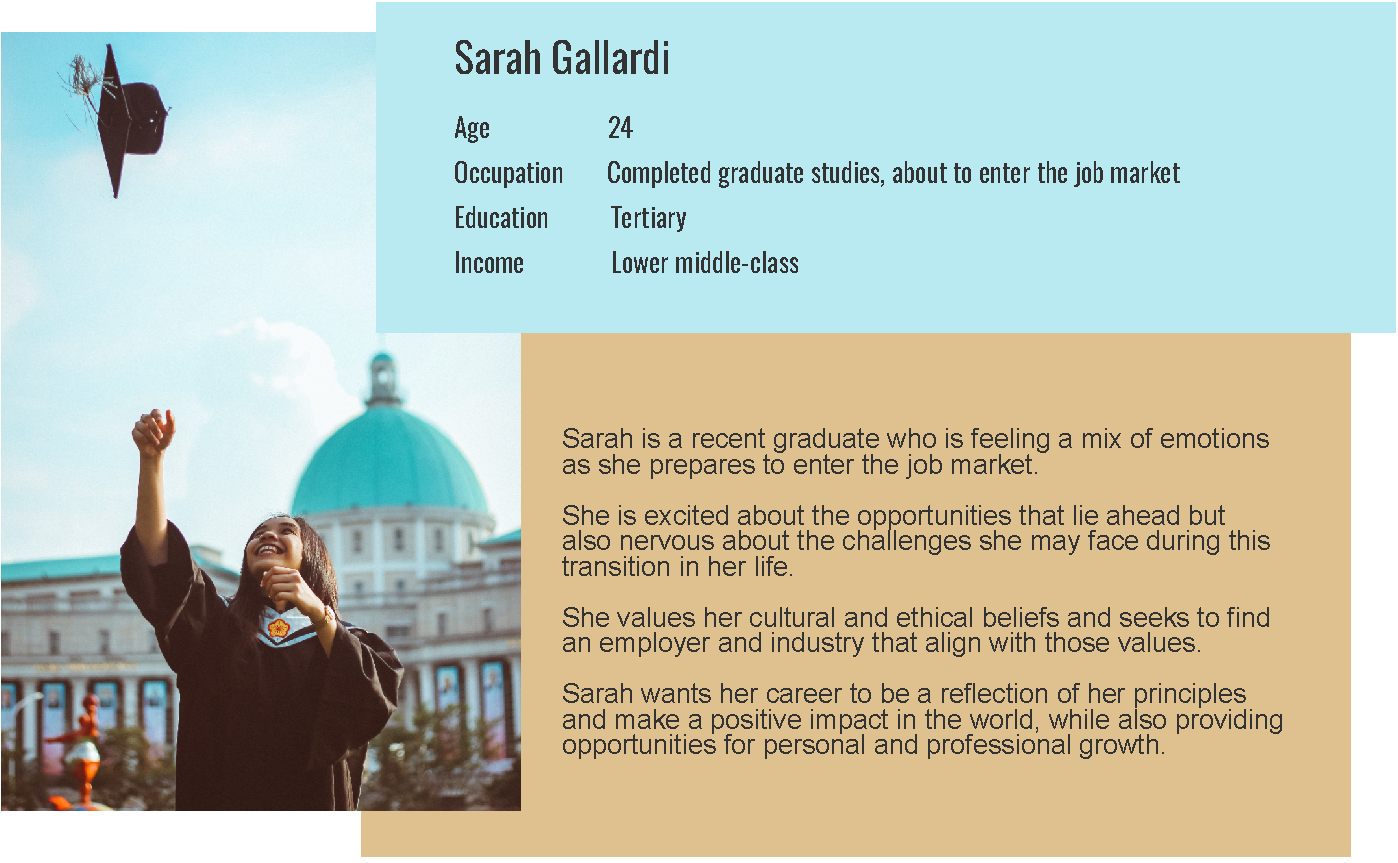
\includegraphics[width=\linewidth]{persona.pdf}
\end{figure}

\noindent\textbf{Goals and Needs:}
Sarah has a number of goals and needs that she wants to achieve and where career counseling could be beneficial to
her. These goals and needs are described in the following, while we try to analyze them in terms of intrinsic and
extrinsic motivation and the hierarchy of needs.

\begin{itemize}
    \item \textbf{Personal advice:}
        Foremost, Sarah wants to receive personalized advice and coaching. She wants to discuss her career goals and plans with a
        professional career counselor. In particular, she wants to learn what career paths are available to her and how she can best
        achieve her career goals. [extrinsic motivation, i.e., higher remuneration, career advancement]
    \item \textbf{Cultural and Ethical Alignment:}
        Sarah places a high value on cultural and ethical alignment with potential employers and industries. She would not want to work 
        in an industry that exploits workers (such as some mining companies), or in the fossil fuels, tobacco or armament industries. She
        dreams of working for a company that promotes diversity, inclusion, equality and respects different perspectives and cultures.
        [intrinsic motivation, self-esteem, belonging, self-actualization]
    \item \textbf{Sustainable Practices:} 
        One particular value Sarah cherishes is sustainability. She wants to work in an industry that is environmentally responsible and
        prioritizes sustainable practices. Through her commitment to sustainability, she hopes to contribute to a better world. [intrinsic
        motivation, self-esteem]
        \item \textbf{Work-Life Balance:}
        Sarah recognizes the importance of work-life balance in maintaining her well-being and overall satisfaction. She prefers
        employers and industries that prioritize a healthy work-life balance, offer flexible working arrangements, and support
        employee well-being initiatives. [intrinsic, self-actualization]
    \item \textbf{Learning and Development:}
        Sarah wants to be challenged in her job, and she seeks continuous learning and development. She values career paths and organizations
        opportunities for professional growth, such as through training programs, mentorships, and support for employees' career advancement.
        [extrinsic, i.e., higher remuneration through career advancement and intrinsic, i.e., self-esteem and self-actualization]
    \item \textbf{Job Security:}
        Like many white collar workers, Sarah is very worried due to the rapid raise of AI technologies. Is her education still going to
        be relevant in five years from now? Will she be replaced by a robot? She wants to find a job that is future-proof and where she
        can build a long-term career. [extrinsic, i.e., basic needs, safety]
\end{itemize}

\noindent\textbf{Summary:}
Overall, Sarah wants to find an employer and industry that not only align with her cultural and ethical values but also provide
opportunities for personal and professional growth. She aspires to contribute to a sustainable, socially responsible, and inclusive
work environment where she can make a positive impact for the world while also thriving in her career. Considering Maslow's hierarchy of needs,
Sarah is currently in the process of fulfilling her basic needs by seeking an employment that will secure food, shelter, etc. through the 
stable remuneration. However, she also has higher aspirations: she strives to fulfill her needs relating to self-esteem, belongingness, and
morality. The right job with the right employer will provide her with a sense of belonging and self-esteem. She wants to feel valued and
appreciated for her contributions, while being able to advance her career within a few years. Finally, aligning her cultural and ethical
values with her career choices will allow her to partly fulfill her self-actualization needs.
\vspace*{0.3cm}

\subsection{Drivers}

Drivers are the set of intrinsic and extrinsic motivators that ultimately drive the behavior of our customers.
These are the deeply-rooted, sometimes unconscious, causes and the true source of the customer's needs. Understanding
these drivers can help us to conceptualize innovative solutions and business models that are more likely to succeed due
to the customer-centricity and acceptance. We will first introduce human drivers that we derive from Maslow's hierarchy
of needs \cite{maslowTheoryHumanMotivation1943} and then discuss customer drivers that are more specific to our
customer segments.

\subsubsection{Human Drivers}

Based on Maslow's hierarchy of needs \cite{maslowTheoryHumanMotivation1943}, we can derive a set of human drivers that
are common to all humans. These drivers are the fundamental motivators that drive human behavior and are therefore
important to consider when designing solutions and business models in career counseling. The needs that are lower in
the hierarchy are more fundamental and must be fulfilled before the higher-level needs.
Figure \ref{fig:maslow} illustrates the hierarchy of needs with examples of specific needs for each level of the pyramid.
In terms of career counseling, we can identify basic physiological needs, such as food and shelter, as well as safety needs,
such as job security, financial security and access to health services as the basic human drivers. Humans strive for employment
to earn an income that helps them to cover their basic physiological needs. Career counseling can guide them to achieve more
safety through a stable employment, career development perspectives leading to increased responsibility and better paid jobs,
thereby increasing income and financial security.

\begin{figure}[h!]
    \centering
    \caption{Human drivers according to Maslow's hierarchy of needs \cite{maslowTheoryHumanMotivation1943} (reproduced
    from Wikimedia Commons under CC-BY license).}
    \label{fig:maslow}
    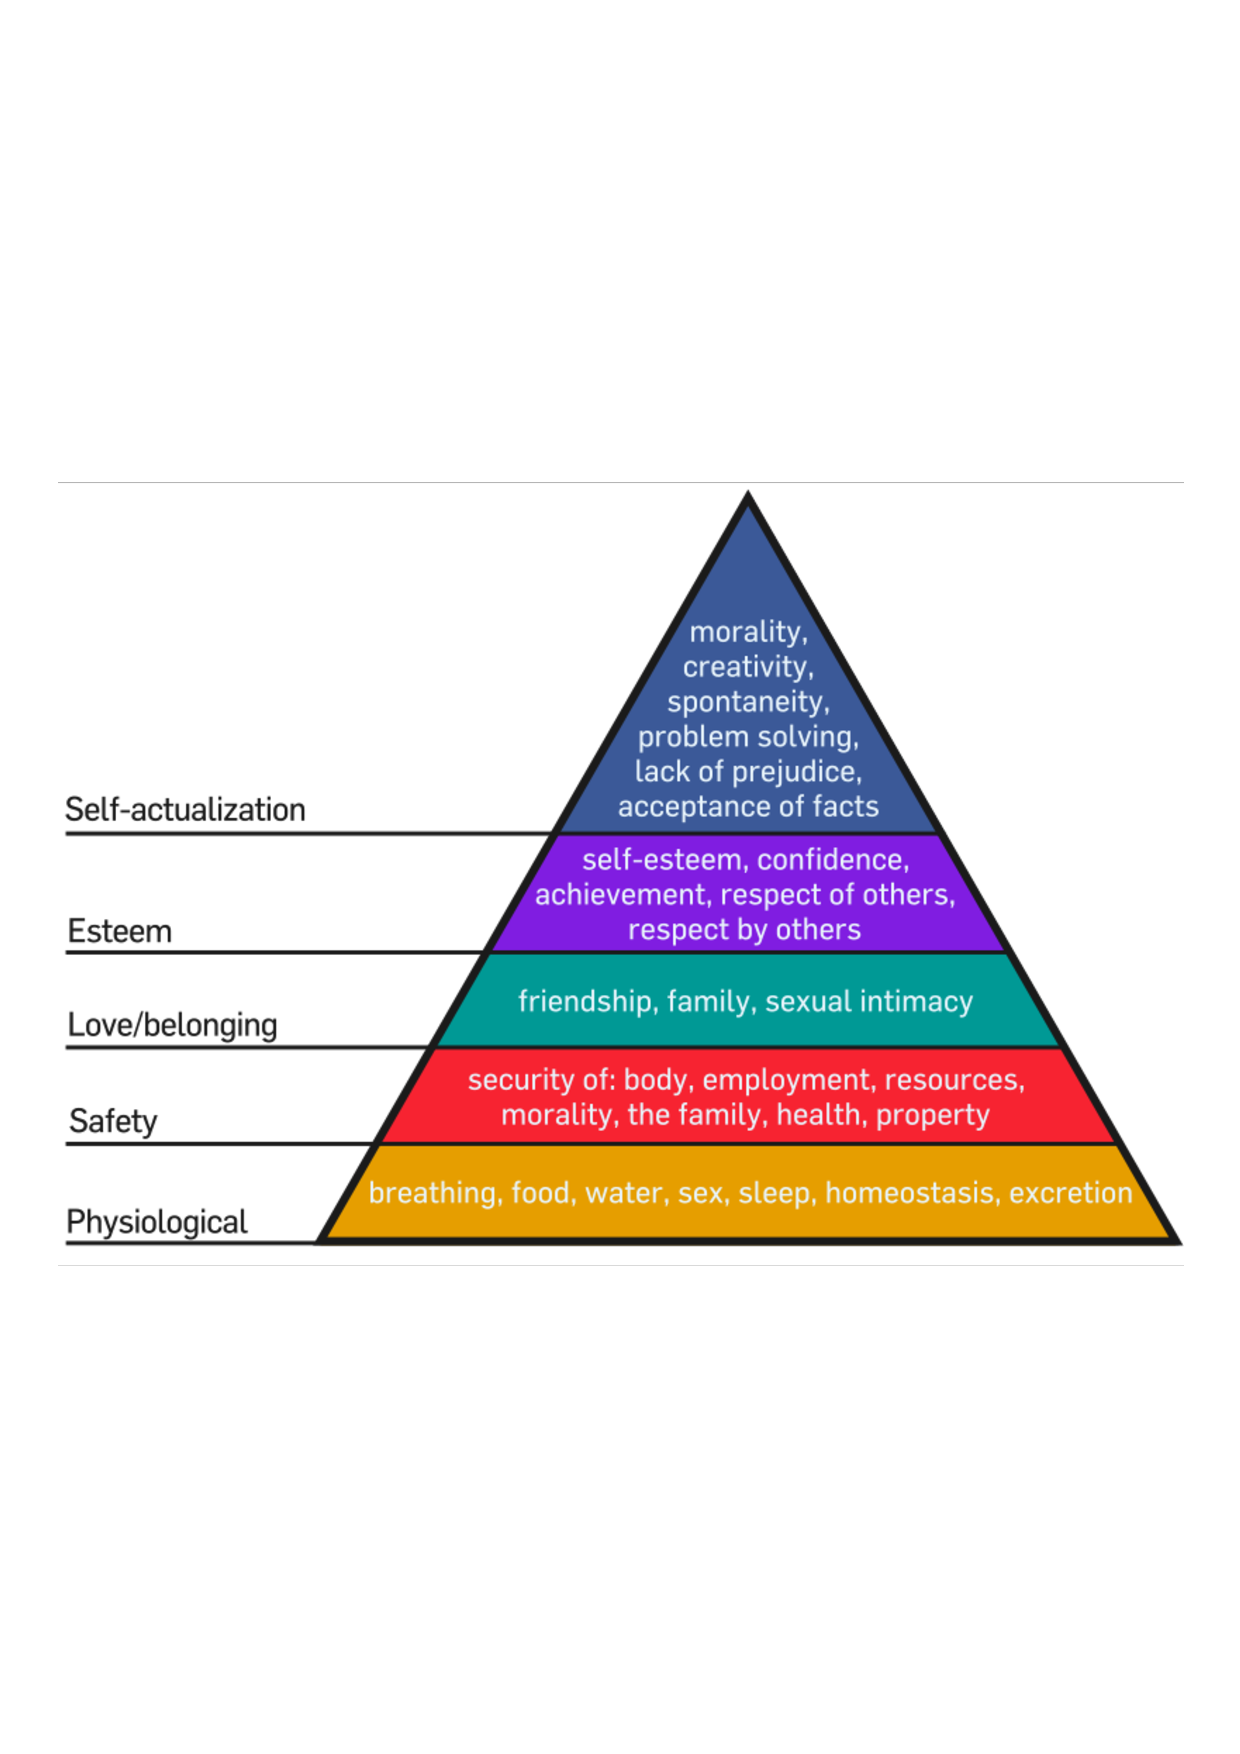
\includegraphics[width=0.8\linewidth]{maslow.pdf}
\end{figure}

\subsubsection{Customer Drivers}

On a higher level of the Maslow pyramid, we can identify a number of customer drivers that guide customers in terms of
demand for career counseling services. These drivers are more specific to our customer segments and are therefore 
highly relevant when designing innovative solutions and business models in career counseling. Based on the persona 
introduced in the previous section, we can identify several customer drivers related to belongingness, self-esteem
and even to self-actualization. A career generates feeling of belongingness by actively participating in the society
and work environment. The goal of a career plan is to advance in life to reach higher-level goals. Through
career advancement, customers achieve higher incomes, reach higher social status, gain more recognition and progressively
build self-confidence and self-esteem. Through an advancement in career, customers are also in a better position to
choose employers and industries they see better fit with their own beliefs and values. This cultural and ethical
alignments allows them to fulfill their self-actualization needs by better exploiting their full potential. In
the case of our persona Sarah, this would translate to her ability to contribute to a better world through
working, e.g., in a sustainable industry.

\subsection{Value Proposition}


The value proposition of a business represents the value that is expected to be generated and delivered to the
customer. Tools like the value proposition canvas, which was introduced by \cite{osterwalderValuePropositionDesign2014},
can help entrepreneurs design effective value propositions. However, the value proposition canvas may not fit very well
for the business model of digital platforms, where value is co-created by different stakeholders and the operator is not
in control of the transactions between different stakeholders of the platform \citep{belleflammeMultisidedValueProposition2021}.
Because of the value co-creation and lack of transactional control, so they continue to argue, it is not clear to whom
the value proposition should specifically be addressed to. Counseling clients are not interested in the matchmaking
and recommendation infrastructure of the platform, but rather in the value that is created by the other users (e.g.,
counselors) and insights from the aggregate data of other users (e.g., career paths). To help digital platforms design
effective value propositions, \cite{belleflammeMultisidedValueProposition2021} proposed the Multisided Value Proposition
Canvas (MVPC). Based on the platform aspect of CCaaS we will thus analyze the customer side based on the perspective of career
counseling clients, but stick to the well-established canvas introduced by \cite{osterwalderValuePropositionDesign2014}. We
consider these counseling clients as the ultimate beneficiaries of the value proposition. Figure~\ref{fig:vpc_customer}
summarizes the customer side of the canvas. In the following we elaborate on the customer jobs that customers are trying
to get done via career counseling services, the pains they experience, and the potential gains that they are seeking
(but that may not be delivered by current offerings).

\subsubsection{Customer Jobs}

Customer jobs represent the tasks that customers are trying to get done as part of career counseling.

\begin{itemize}
    \item Find a job that matches with education, skills, culture and ethical values
    \item Learn skills that are relevant in the job market and future-proof
    \item Grow on a personal and professional level
    \item Achieve rapid career advancement
    \item Steadily increase role and responsibility
    \item Steadily increase income
    \item Successfully navigate career changes
\end{itemize}

\subsubsection{Pains}

Pains represent the negative emotions, costs, and risks that customers are regularly experience before
or during getting their customer jobs done within career counseling.

\begin{itemize}
    \item Career counseling is expensive
    \item Career counselors have only limited time to spend with each customer
    \item Based on limited previous experience, some career counselors may not be able to provide
        good advice based on the customer's individual profile (a single counselor may have only
        seen a limited amount of similar cases and career transitions to provide effective advice)
\end{itemize}

\subsubsection{Gains}

Gains represent the benefits that customers would wish from career counseling services but are 
typically not part of the current offering.

\begin{itemize}
    \item Truly personalized coaching and career planning
    \item Insights into common career paths and career transitions given the customer's profile
    \item 24/7 access to career counseling
\end{itemize}

\begin{figure}[h!]
    \centering
    \caption{The customer side of the Value Proposition Canvas for career counseling services (background illustration adapted from Strategyzer.com).}
    \label{fig:vpc_customer}
    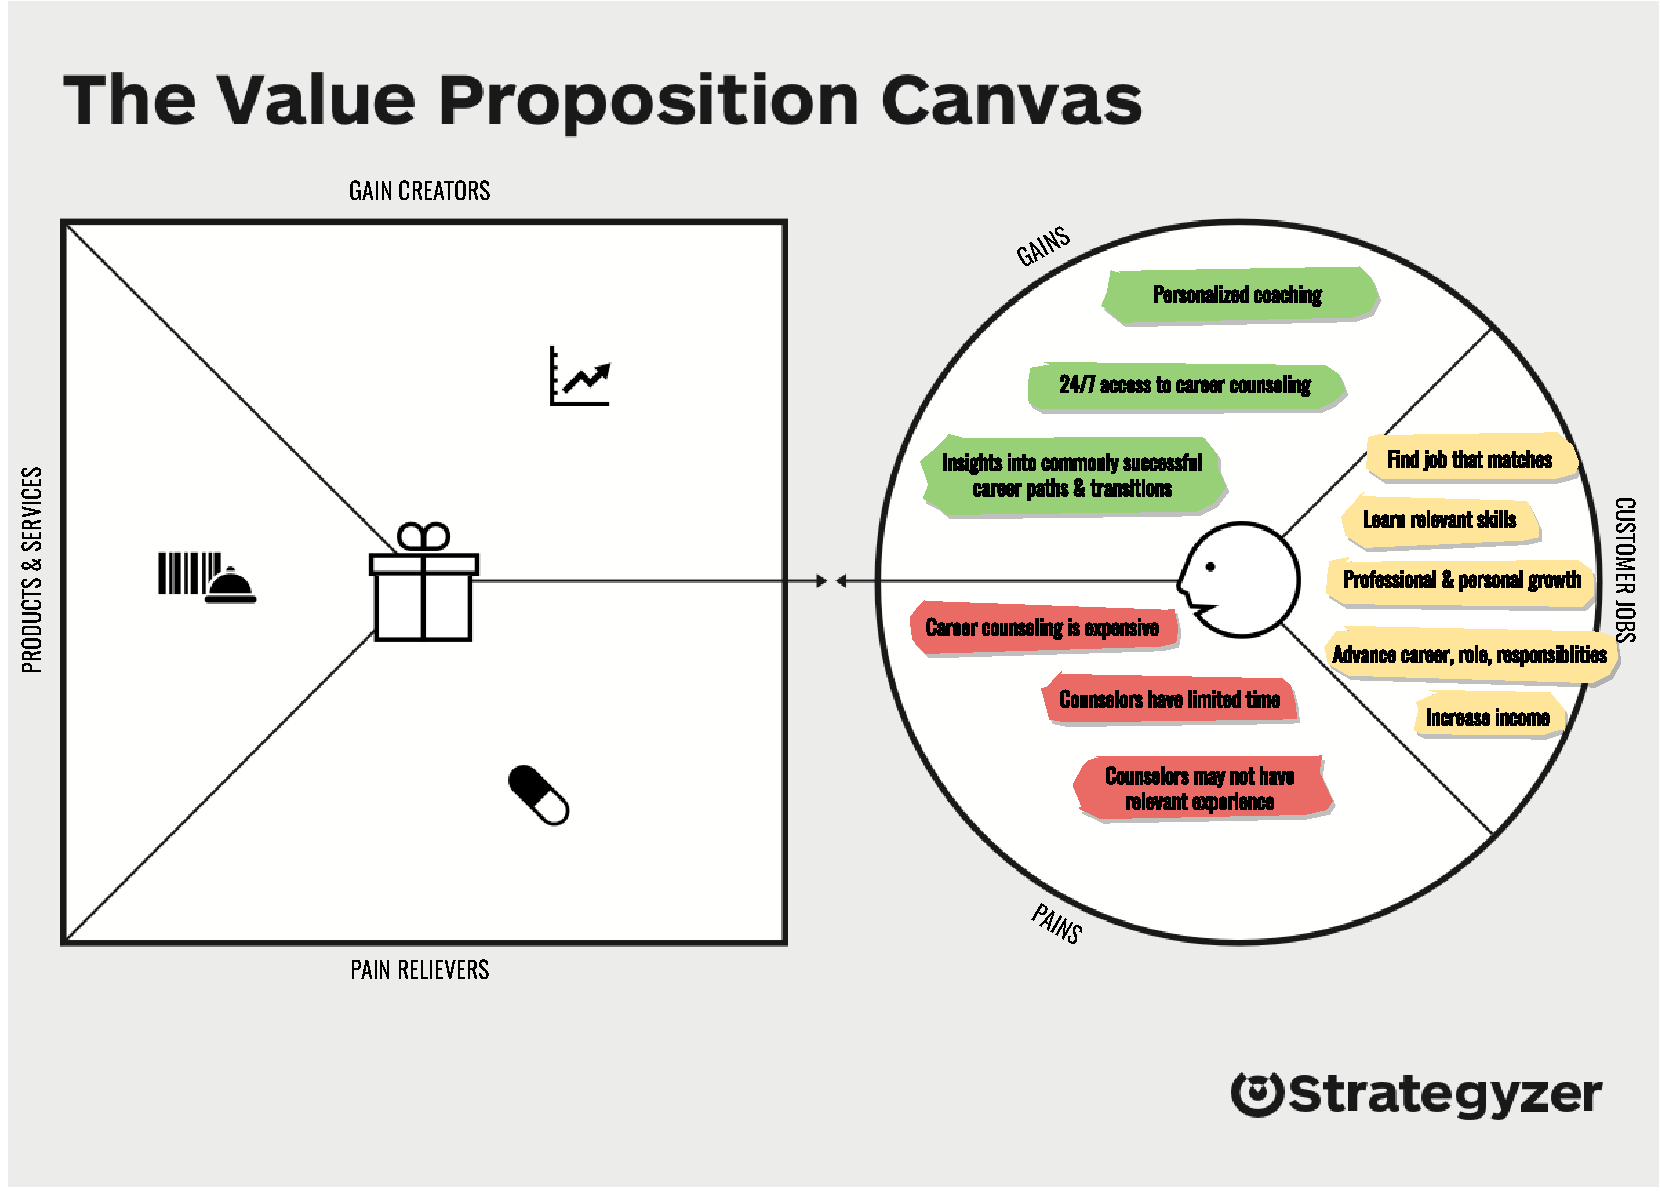
\includegraphics[width=\linewidth]{vpc_customer.pdf}
\end{figure}

\noindent In Section \ref{sec:enablers} we will introduce the value proposition canvas and enablers from the
side of the innovating company, i.e., LinkedIn.